{%	---------------------------- Apresentacao -----------------------------------	%
%																					%
%	Desenvolvendo um modelo padrao para trabalhos academicos utilizando o ABNTeX2	%
%	Autor: Salomão Luiz de Araújo Neto												%
%	GitHub:	https://github.com/salomaoluiz											%
%	LinkedIn: https://www.linkedin.com/salomao-luiz									%
%																					%
%	-----------------------------------------------------------------------------	%
}

{%	------------------------ Informacoes de Uso ---------------------------------	%
%																					%
%	1. Nao e utilizado acentuacao nas areas de comentario para evitar crash de	 	%
%	texto ao ser utilizado em outro sistema, tornando os comentarios ilegiveis.		%
%																					%
%	2. Ao utilizar este documento, por gentileza de creditos ao autor, com isto		%
%	o seu e o meu trabalho sao valorizados.											%
%																					%
%	3. Realize as modificacoes que achar necessario, seja para adequar aos pedidos	%
%	de sua universidade, ou por gosto proprio, mas caso queira realizar uma 		%
%	contribuicao com o codigo, o mantenha sempre comentado, para um melhor			%			
%	entendimento.																	%
%																					%	
%	4. Softwares Utilizados: TeXstudio e MikTeX, sempre que for compilar seu		%
%	projeto, tenha certeza de possuir conexao com a internet, para que seja 		%
%	possivel o download dos pacotes necessarios.									%
%																					%
%	5. A tela utilzada para a elaboracao deste projeto foi uma 1366x768, recomendo	%
%	a utilizacao de uma de igual ou maior resolucao para nao haver bagunca no		%
%	desing do projeto.																%
%	-----------------------------------------------------------------------------	%
}

%	-----------------------------------------------------------------------------	%
%	---------------------------	Inicio do Preambulo	-----------------------------	%
%	-----------------------------------------------------------------------------	%

\documentclass[	12pt,								%Tamanho da Fonte
openright,							%Abre a Direita
twoside,							%Imprime Frente/Verso
a4paper,							%Folha A4
chapter = TITLE,					%Capitulos em Maiusculo
section = TITLE,					%Secoes em Maiusculo
subsection = TITLE,					%Subsecoes em Maiusculo
subsubsection = TITLE,				%Subsubsecoes em Maiusculo
english, french, spanish, brazil]	%Idiomas Usados
{abntex2}

%	-----------------------------------------------------------------------------	%
%	---------------------------	Pacotes Utilizados	-----------------------------	%
%	-----------------------------------------------------------------------------	%

\usepackage{./lib/unemaTeX	}


%	-----------------------------------------------------------------------------	%
%	-----------------------	Informacoes do Trabalho -----------------------------	%
%	-----------------------------------------------------------------------------	%

%%%%%%%%%%%%%%%%%%%%%%%
%% Dados do Trabalho %%
%%%%%%%%%%%%%%%%%%%%%%%	
\titulo{Desenvolvimento unemaTeX}
\autor{Salomão Luiz de Araújo Neto}
\tipotrabalho{Monografia}
\orientador[Profº Dr. ]{Nome Orientador}
\coorientador[Profº Dr.]{Nome Coorientador}
\local{Sinop, MT}
\data{2018}

\professorconvidadoum{Convidado Um}
\professorconvidadodois{Convidado Dois}


%%%%%%%%%%%%%%%%%%%%%%%%%%
%% Dados da Instituicao %%
%%%%%%%%%%%%%%%%%%%%%%%%%%
\faculdade{Faculdade de Ciências Exatas e Tecnológicas}
\departamento{Departamento de Matemática}
\campus{Campus de Sinop - MT}
\curso{Licenciatura em Matemática}
\titulocurso{Licenciado} %pode ser 'Bacharel'
\resumocurso{Matemática}


	
%	-----------------------------------------------------------------------------	%
%	---------------------------	Inicio do Documento -----------------------------	%
%	----------------------------------------------------------------------------	%	
\begin{document}

%	-------------------------- Elementos Pre-Textuais ---------------------------	%
\imprimircapa
\imprimirfolhaderosto*{}
\begin{fichacatalografica}
	\sffamily
	\vspace*{15cm}		%Posicao Vertical

	\begin{center}
		INSERIR FIGURA DA FICHA CATALOGRÁFICA AQUI
	\end{center}
\end{fichacatalografica}
%\begin{errata}
	FERRIGNO, C. R. A. \textbf{Tratamento de neoplasias ósseas apendiculares
	com
	reimplantação de enxerto ósseo autólogo autoclavado associado ao plasma
	rico em plaquetas}: estudo crítico na cirurgia de preservação de membro em
	cães. 2011. 128 f. Tese (Livre-Docência) - Faculdade de Medicina
	Veterinária
	e Zootecnia, Universidade de São Paulo, São Paulo, 2011.
	\begin{table}[htb]
		\center
		\footnotesize
		\begin{tabular}{|p{1.4cm}|p{1cm}|p{3cm}|p{3cm}|}
			\hline
			\textbf{Folha} & \textbf{Linha} & \textbf{Onde se lê} &
			\textbf{Leia-se}\\
			\hline
			1 & 10 & auto-conclavo & autoconclavo\\
			\hline
		\end{tabular}
	\end{table}
\end{errata}
%	-------------- Utilizar Isto Quando conseguir a folha de Aprovacao --------------	%
%\includepdf{./arquivos/folhaAprovacaoFinal.pdf}

%	---------------------- Utilizar Isto de Forma Temporaria -----------------------	%
\begin{folhadeaprovacao}
	\begin{center}
		{\ABNTEXchapterfont\large\imprimirautor}
		\vspace*{\fill}\vspace*{\fill}
		\begin{center}
			\ABNTEXchapterfont\bfseries\Large\imprimirtitulo
		\end{center}
		\vspace*{\fill}
		\hspace{.45\textwidth}
		\begin{minipage}{.5\textwidth}
			\imprimirpreambulo
		\end{minipage}%
		\vspace*{\fill}
	\end{center}
	Trabalho aprovado. \imprimirlocal, 24 de novembro de 2012:
	\assinatura{\textbf{\imprimirorientador} \\ Orientador}
	\assinatura{\textbf{Professor} \\ Convidado 1}
	\assinatura{\textbf{Professor} \\ Convidado 2}
	\begin{center}
		\vspace*{0.5cm}
		{\large\imprimirlocal}
		\par
		{\large\imprimirdata}
		\vspace*{1cm}
	\end{center}
\end{folhadeaprovacao}
\begin{dedicatoria}

\textodedicatoria{Agradeço ao mundo por sempre evoluir ao seu tempo e sua maneira, pois assim não teríamos o que pesquisar, o que descobrir e o que nos motivar a viver. Por seus mistérios, ainda não desvendados e pelas pessoas que habitam nele, pois através disto consegui ter considerações finais sobre muitos conceitos, não somente deste trabalho, mas para futuras "diversões"}

\imprimirdedicatoria
\end{dedicatoria}
\begin{agradecimentos}

Agradeço à...

\end{agradecimentos}
\begin{epigrafe}
\vspace*{\fill}


\begin{flushright}
	\begin{minipage}{7cm}
	\end{minipage}
	\begin{minipage}{7cm}
		\flushright
		\textit{O mundo é um lugar perigoso de se viver, não por causa daqueles que fazem o mal, mas sim por causa daqueles que observam e deixam o mal acontecer.\\
		\textbf{Albert Einstein}}
	\end{minipage}
\end{flushright}

\end{epigrafe}
\begin{resumo}

Resumo em Português

\vspace{\onelineskip}
\noindent
\textbf{Palavras-chave}: latex. abntex. editoração de texto.

\end{resumo}
\begin{resumo}[Abstract]
	\begin{otherlanguage*}{English}
		Abstract in English
		
		\vspace{\onelineskip}
		\noindent
		\textbf{Keywords}: latex. abntex. text publisher.
		
	\end{otherlanguage*}
\end{resumo}
\begin{resumo}[Résumé]
	\begin{otherlanguage*}{french}
		Il s'agit d'un résumé en français
		
		\vspace{\onelineskip}
		\noindent
		\textbf{Mots-clés}: latex. abntex. publication de textes.
		
	\end{otherlanguage*}
\end{resumo}

\listoffigures*
\cleardoublepage
\listoftables*
\cleardoublepage

\begin{siglas}
	\item[ABS] Acrylonitrile Butadiene Styrene
	\item[PLA] Ácido Polilático
\end{siglas}
\begin{simbolos}
	\item[ºC] Graus Célcios
	\item[ºF] Graus Fahrenheit
	\item[$\gamma$] Letra Grega Gamma
	\item[$\Lambda$] Letra Grega Lambda
\end{simbolos}
\tableofcontents*

	%	--------------------- Elementos Textuais -----------------------	%

\mainmatter
\chapter*{Introdução}
\addcontentsline{toc}{chapter}{INTRODUÇÃO}
Neste trabalho é utilizado da plataforma LaTeX para o desenvolvimento de um modelo acadêmico para Projetos de Pesquisa, Trabalhos de Conclusão de Curso entre outros tipos, para a utilização na Universidade do Estado de Mato Grosso, Campus Sinop.

Tem-se com intuito deste possibilitar a facilidade e a padronização dos trabalhos acadêmicos, permitindo que qualquer um com um conhecimento básico em desenvolvimento TeX consiga elaborar um trabalho com uma excelente tipografia. Neste trabalho será mostrado como pode ser utilizado para a inserção de tabelas, figuras, equações, bibliografia, tudo dentro das normas da ABNT.


\chapter{Softwares Utilizados}

\section{MikTeX}
\section{TeXstudio}
\subsection{Principais Características do TeXstudio}
\chapter{Configurações do Preâmbulo}
\section{Configurações do \textbackslash documentclass}
O \lstinline|\documentclass{}| é uma das configurações básicas de um documento \LaTeX, nele é onde é definido as principais características do documento, como se sera um trabalho acadêmico, um artigo, banner ou slide. Por ele é possível configurar os padrões do documento, como tamanho de fonte ou da folha, a linguagem, configurações de titulo e subtítulos.

As configurações utilizadas no \lstinline|\documentclass{}| foram:
\begin{itemize}
	\item 12pt $\rarrow$ Tamanho de Fonte 12												
	\item openright $\rarrow$ Inicia a pagina pela direita										
	\item twoside $\rarrow$ A pagina sera impressa frente e verso
	\item a4paper $\rarrow$ O papel padrão com tamanho A4									
	\item brazil $\rarrow$ Define a linguagem com Português-Brasil							
	\item abntex2 $\rarrow$ Para utilizar a classe do documento com normas ABNT				
\end{itemize}


\chapter{Etapa Textual}
\section{Capítulos, Seções e Subseções}


\section{Equações e Simbologia Matemática}
Apesar da plataforma de desenvolvimento LaTeX poder ser utilizado por qualquer ramo da ciência para o desenvolvimento de trabalhos com uma excelente tipografia, ela é principalmente utilizada por pessoas das áreas exatas, por conta da enorme facilidade em desenvolver trabalhos com enormes quantidades de equações e fórmulas, com estas se mantendo sempre organizadas. Para fazer a inserção de equações, funções ou simbologia matemática é preciso estar dentro do ambiente matemático, este é uma área apenas para a inserção de fórmulas matemáticas. 

Este espaço pode ser feito de duas formas, dentro do texto, ou em um ambiente separado. Para a utilização dentro do texto, as equações matemáticas precisam ser inseridas dentro de um par de \$, por exemplo \$ 3x\textasciicircum 2 = 2 \$, ao usar essa forma, o código fica da seguinte maneira: $3x^2=2$.

Outra forma de se adicionar fórmulas, funções ou símbolos matemáticos é pelo ambiente \lstinline[language=TeX]|\begin{equation} \end{equation}| tudo que se colocar dentro destas funções será centralizado, enumerado, e ficará em formato matemático. Por exemplo, ao usar:
\begin{lstlisting}[language=TeX]
\begin{equations}\label{equacao1}
	3x^2 = 2
\end{equations}
\end{lstlisting}
tem-se como resultado:

\begin{equation}\label{equacao1}
	3x^2 = 2
\end{equation}
\
Está forma é muito útil quando você quer referenciar alguma equação ao longo do texto, pois com o comando \lstinline[language=TeX]|\label{}| você pode em qualquer local utilizar o \lstinline[language=TeX]|\ref{}| para referenciar aquele ``label'', por exemplo: ``Seja a equação \ref{equacao1} tem-se que...'' é possível fazer isso para todas as equações dentro do ambiente ``equation'', figuras, tabelas, basta alterar o que está escrito dentro do ``label'', e usar o ``ref'' para referenciar ela.

Outra forma de inserir equações matemáticas é utilizando \lstinline[language=TeX]|\[ \]| o que colocar dentro destes colchetes será centralizado, mas não sera enumerado, por exemplo:
\begin{lstlisting}
\[
3x^2=2
\]
\end{lstlisting}
terá como resultado:
\[
3x^2=2
\]
\subsection{Simbologia Matemática}
O LaTeX possui suporte a diversos símbolos matemáticos, desde simbologia como $\pm \div \bullet \bigtriangleup \neq \gg$ como também letras gregas como $\beta \gamma \delta \epsilon \varepsilon$ entre muitos outros. Para ver todos os símbolos matemáticos vá em ``View'' em ``Show'' e selecione ``Side Panel'', com isso irá abrir uma tela no canto lateral, navegue por ela e veja todos os símbolos que se pode adicionar, sempre fique atento em colocar os símbolos dentro de um ambiente matemático, se não será impossível compilar o projeto.
\subsection{Trabalhando com Equações}
O LaTeX tem suporte a diversas funções matemáticas, e alguns comandos que possibilitam o melhoramento dessas equações, a tabela

\begin{table}[htb]
	\IBGEtab{%
		\caption{Algumas Funções Matemáticas}%
		\label{tab_Cap2_equacoes}
	}{%
	\begin{tabular}{ccc|ccc}
		\toprule
		     Equação      &                   Código                    &      Resultado       &       Equação       &                Código                &     Resultado     \\ \midrule\midrule
		  Raiz Quadrada   &                \ba sqrt\{x\}                &      $\sqrt{x}$      & Integral Indefinida &             \ba int\{x\}             &     $\int{x}$     \\
		Raiz a Potencia N &              \ba sqrt[3]\{x\}               &    $\sqrt[3]{x}$     &  Integral Definida  & \ba int\_{2}\textasciicircum{3}\{x\} & $\int_{2}^{3}{x}$ \\
		    Somatoria     & \ba sum\_\{i=1\}\textasciicircum\{10\}\{x\} & $\sum_{i=1}^{10}{x}$ &       Fração        &          \ba frac\{x\}\{y\}          &   $\frac{x}{y}$   \\ \bottomrule
	\end{tabular}%
}{%
\fonte{Autoria Própria}%
}
\end{table}

Muitas outras funções podem ser obtidas indo em ``Math'' e em ``Math Function''. Observe que quando se utiliza uma função complexa dentro de uma tabela, como por exemplo a somatória, ela fica com a aparência um pouco ruim, com pouca organização, para resolver este problema, basta colocar antes da equação o comando \lstinline[language=TeX]|\displaystyle| assim ela ficará da seguinte forma:
\[
\sum_{i=1}^{10}{x}
\]

O mesmo vale para integrais, frações, raízes, entre outras.
\subsection{Tabulações}
\subsubsection{Matrizes}
Para a criação de matrizes existem os ambientes ``pmatrix'', ``bmatrix'', ``vmatrix'', ``Vmatrix'', ``matrix'' e ``array''. O ``pmatrix'' serve para a criação de matrizes com parenteses nas bordas, como por exemplo:
\[
\begin{pmatrix}
	2x & 3x \\ 
	x & 4x
\end{pmatrix} 
\]

o ``bmatrix'' serve para criar matrizes na forma de caixa, por exemplo:
\[
\begin{bmatrix}
2x & 3x \\ 
x & 4x
\end{bmatrix} 
\]

o ``vmatrix'' e o ``Vmatrix'' servem para criar matrizes com barras nas bordas, o primeiro com 1 barra, e o segundo com 2 barras, por exemplo: \\
\begin{center}
$
\begin{vmatrix}
2x & 3x \\ 
x & 4x
\end{vmatrix} 
$
\hspace*{2cm}
$
\begin{Vmatrix}
2x & 3x \\ 
x & 4x
\end{Vmatrix} 
$
\end{center}

o ``matrix'' cria uma matriz sem nenhuma borda
\[
\begin{matrix}
2x & 3x \\ 
x & 4x
\end{matrix}
\]

já o ``array'' é possível editar para colocar barras entre cada coluna ou linha, por exemplo:
\[
\begin{array}{c|ccc}
2x & 3y &2z & 4w\\ 
x & 4y & 3z & 8w \\ \hline
3x & 7y & 5z & 12w
\end{array}
\]
é possível também colocar o array dentro de um ``bmatrix'', ou ``pmatrix'' ou qualquer outra matriz, mas caso você deseje utilizar por exemplo, um lado de parentese e outro de colchete, é preciso usar as funções \lstinline[language=TeX]|\left| e \lstinline[language=TeX]|\right| acompanhado do simbolo que deseje, por exemplo:
\begin{lstlisting}[language=TeX]
\[
 \left[
  \begin{array}{c|ccc}
  2x & 3y &2z & 4w\\ 
  x & 4y & 3z & 8w \\ \hline
  3x & 7y & 5z & 12w
  \end{array}
 \right)
\]
\end{lstlisting}
que fornece como resultado:
\[
\left[
\begin{array}{c|ccc}
2x & 3y &2z & 4w\\ 
x & 4y & 3z & 8w \\ \hline
3x & 7y & 5z & 12w
\end{array}
\right)
\]

\subsubsection{Tabelas}
Para a utilização de Tabelas nas normas da ABNT é preciso usar os comandos:




\begin{lstlisting}
\begin{table}[htb]
\IBGEtab{%
\caption{Aqui vai o titulo da tabela}%
\label{tab_Cap2_exemplo}
}{%
\begin{tabular}{ccc}
	\toprule
	     Nome       &     Cidade     &    Estado    \\ \midrule\midrule
	Pedro da Silva  &     Cuiaba     & Mato Grosso  \\
	  Joao Neves    &   Sao Paulo    &  Sao Paulo   \\
	Maria Antonieta & Belo Horizonte & Minas Gerais \\ \bottomrule
\end{tabular}%
}{%
\fonte{Autoria Propria}%
\nota[Nota1]{Aqui pode ser inserido uma nota sobre a tabela}
}
\end{table}
\end{lstlisting}

Isto fornece a seguinte tabela:
\begin{table}[htb]
\IBGEtab{%
\caption{Aqui vai o titulo da tabela}%
\label{tab_Cap2_exemplo}
}{%
\begin{tabular}{ccc}
	\toprule
	     Nome       &     Cidade     &    Estado    \\ \midrule\midrule
	Pedro da Silva  &     Cuiaba     & Mato Grosso  \\
	  João Neves    &   São Paulo    &  São Paulo   \\
	Maria Antonieta & Belo Horizonte & Minas Gerais \\ \bottomrule
\end{tabular}%
}{%
\fonte{Autoria Própria}%
\nota[Nota1]{Aqui pode ser inserido uma nota sobre a tabela}
}
\end{table}


\subsection{Apresentação de Códigos de Programação}

\section{Inserção de Imagens}
Para adicionar imagens, conforme as normas da ABNT, é necessário utilizar o código:
\begin{lstlisting}[language=TeX]
\begin{figure}[htb]			
  \caption{Brasao Unemat \label{fig_Cap2_brasaoUnemat}}
  \begin{center}
    
\includegraphics[scale=0.1]{./Imagens/Brasao_Unemat.png}
  \end{center}
  \legend{Fonte: http://sinop.unemat.br/site/}
\end{figure}
\end{lstlisting}

Com este código, a imagem fica na seguinte forma:

\begin{figure}[htb]			
	\caption{Brasão Unemat \label{fig_Cap2_brasaoUnemat}}
	\begin{center}
		
\includegraphics[scale=0.1]{./Imagens/Brasao_Unemat.png}
	\end{center}
	\legend{Fonte: http://sinop.unemat.br/site/}
\end{figure}
\chapter{Elementos Pós Textuais}
\section{Bibliografia}

Para criar um bibliografia, vá na pasta ``bibliografia'' dentro da pasta ``elementosPosTextuais'' e edite o arquivo. Existem vários tipos de bibliografias que se podem utilizar, como por exemplo:

\begin{table}[htb]
	\IBGEtab{%
		\caption{Tipos de Bibliografias}%
		\label{tab_Cap3_bibliografia}
	}{%
		\begin{tabular}{ccc}
			\toprule
			   Tipo    &     Tipo      &     Tipo      \\ \midrule\midrule
			 article   &     book      &    manual     \\
			   www     &    booklet    &   commented   \\
			  inbook   & incollection  & inproceedings \\
			jurthesis  & mastersthesis &     misc      \\
			periodical &   phdthesis   &  proceedings  \\
			techreport &  unpublished  &               \\ \bottomrule
		\end{tabular}%
	}{%
		\fonte{\cite{ferreira}}%
	}
\end{table}

\subsection{Criando uma Referência}
Para criar uma referência, é preciso ir até o arquivo da bibliografia, e dependendo do tipo de referência, alguns elementos precisam ser colocados, por exemplo, ao usar um artigo de referência é preciso colocar:

\begin{figure}[htb]
	\begin{center}
		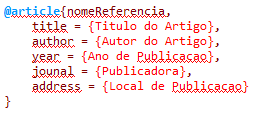
\includegraphics[scale=1]{./Imagens/capitulo_3/code_1.png}
	\end{center}
\end{figure}

Isso irá criar uma referencia, que poderá ser chamada em uma citação utilizando de 3 formas, citações diretas/indiretas curtas e longas, e  citações no texto.

Uma observação quanto a criação de referência, é que em muitas vezes o software não consegue reconhecer acentuações, então é preciso utilizar de comandos para inserir os acentos, os principais comandos são:
\begin{table}[htb]
	\IBGEtab{%
		\caption{Acentuação}%
		\label{tab_Cap3_acentos}
	}{%
		\begin{tabular}{cc}
			\toprule
			         Comando          & Acento \\ \midrule\midrule
			        \ba'\{a\}         &   á    \\
			       \ba ~\{a\}         &   ã    \\
			       \ba `\{a\}         &   à    \\
			\ba\textasciicircum \{a\} &   â    \\
			       \ba c\{c\}         &   ç    \\ \bottomrule
		\end{tabular}%
	}{%
		\fonte{Autoria Própria}%
	}
\end{table}
\subsection{Formas de Citações}
Uma citação direta ou indireta pode ser adicionado no próprio texto, conforme as normas citações com até três linhas, usando \lstinline|\citeonline{nomeReferencia}|. Por exemplo: ``Conforme dito por \citeonline{gajanan} tem-se que...''.

Outra forma de se fazer uma citação é de forma direta curta, como foi utilizado na tabela anterior, para fazer uma citação dessa forma, utiliza-se após a citação o comando \lstinline|\cite{nomeReferencia}|. Por exemplo: ``Existem centenas de estilos bibliográficos mundo a fora.''\cite{araujo2016}

Para citações grandes, com mais de 3 linhas, é preciso utilizar um ambiente especifico para citações longas \lstinline|\begin{citacao} Texto \cite{nomeReferencia}\end{citacao}|. Utilizando deste ambiente, é possível fazer citações da forma:
\begin{citacao}
	Três anos depois de ter anunciado uma descoberta há muito esperada pelos físicos, o bóson de Higgs, a Organização Europeia para a Pesquisa Nuclear (CERN, na sigla em francês) divulga a melhor representação da partícula já capturada até hoje. A imagem, apresentada nesta terça-feira (01/09/2015) durante uma conferência anual da instituição, foi o resultado da combinação dos dados coletados no Grande Colisor de Hádrons por dois experimentos diferentes, o ATLAS e o CMS, entre os anos de 2011 e 2012. \cite{oliveira2015}
\end{citacao}

Exite ainda uma 4º forma de realizar uma citação, mas neste caso, não existe citação em sí, apenas a inserção da referência na lista de bibliografia. Não recomendo utilizar está forma, mas caso seja necessário utilize o comando \lstinline|\nocite{nomeReferencia}|. Por exemplo, irei citar o livro Teorias de Aprendizagem de Marco Antônio Moreira sem apresentar nenhuma citação, apenas adicionando o comando \lstinline|\nocite{moreira2011}|. \nocite{moreira2011}



	%	------------------- Elementos Pós Textuais ---------------------	%
%\bibliography{./elementosPosTextuais/bibliografia/bibliografia}

\end{document}